%% Преамбула TeX-файла

% 1. Стиль и язык
\documentclass[utf8x]{G7-32} % Стиль (по умолчанию будет 14pt)
\usepackage[T2A]{fontenc}
\usepackage[russian]{babel}
% Остальные стандартные настройки убраны в preamble.inc.tex.
\sloppy

% Настройки стиля ГОСТ 7-32
% Для начала определяем, хотим мы или нет, чтобы рисунки и таблицы нумеровались в пределах раздела, или нам нужна сквозная нумерация.
\EqInChapter % формулы будут нумероваться в пределах раздела
\TableInChapter % таблицы будут нумероваться в пределах раздела
\PicInChapter % рисунки будут нумероваться в пределах раздела

% Добавляем гипертекстовое оглавление в PDF
\usepackage[
bookmarks=true, colorlinks=true, unicode=true,
urlcolor=black,linkcolor=black, anchorcolor=black,
citecolor=black, menucolor=black, filecolor=black,
]{hyperref}

% Изменение начертания шрифта --- после чего выглядит таймсоподобно.
% apt-get install scalable-cyrfonts-tex

\IfFileExists{cyrtimes.sty}
    {
        \usepackage{cyrtimespatched}
    }
    {
        % А если Times нету, то будет CM...
    }

\usepackage{graphicx}   % Пакет для включения рисунков

% С такими оно полями оно работает по-умолчанию:
% \RequirePackage[left=20mm,right=10mm,top=20mm,bottom=20mm,headsep=0pt]{geometry}
% Если вас тошнит от поля в 10мм --- увеличивайте до 20-ти, ну и про переплёт не забывайте:
\geometry{right=20mm}
\geometry{left=30mm}


% Пакет Tikz
\usepackage{tikz}
\usetikzlibrary{arrows,positioning,shadows}

% Произвольная нумерация списков.
\usepackage{enumerate}

% ячейки в несколько строчек
\usepackage{multirow}

% itemize внутри tabular
\usepackage{paralist,array}


% Настройки листингов.
% 8 Листинги

\usepackage{listings}

% Значения по умолчанию
\lstset{
  basicstyle= \footnotesize,
  breakatwhitespace=true,% разрыв строк только на whitespacce
  breaklines=true,       % переносить длинные строки
%   captionpos=b,          % подписи снизу -- вроде не надо
  inputencoding=koi8-r,
  numbers=left,          % нумерация слева
  numberstyle=\footnotesize,
  showspaces=false,      % показывать пробелы подчеркиваниями -- идиотизм 70-х годов
  showstringspaces=false,
  showtabs=false,        % и табы тоже
  stepnumber=1,
  tabsize=4,              % кому нужны табы по 8 символов?
  frame=single
}

% Стиль для псевдокода: строчки обычно короткие, поэтому размер шрифта побольше
\lstdefinestyle{pseudocode}{
  basicstyle=\small,
  keywordstyle=\color{black}\bfseries\underbar,
  language=Pseudocode,
  numberstyle=\footnotesize,
  commentstyle=\footnotesize\it
}

% Стиль для обычного кода: маленький шрифт
\lstdefinestyle{realcode}{
  basicstyle=\scriptsize,
  numberstyle=\footnotesize
}

% Стиль для коротких кусков обычного кода: средний шрифт
\lstdefinestyle{simplecode}{
  basicstyle=\footnotesize,
  numberstyle=\footnotesize
}

% Стиль для BNF
\lstdefinestyle{grammar}{
  basicstyle=\footnotesize,
  numberstyle=\footnotesize,
  stringstyle=\bfseries\ttfamily,
  language=BNF
}

% Определим свой язык для написания псевдокодов на основе Python
\lstdefinelanguage[]{Pseudocode}[]{Python}{
  morekeywords={each,empty,wait,do},% ключевые слова добавлять сюда
  morecomment=[s]{\{}{\}},% комменты {а-ля Pascal} смотрятся нагляднее
  literate=% а сюда добавлять операторы, которые хотите отображать как мат. символы
    {->}{\ensuremath{$\rightarrow$}~}2%
    {<-}{\ensuremath{$\leftarrow$}~}2%
    {:=}{\ensuremath{$\leftarrow$}~}2%
    {<--}{\ensuremath{$\Longleftarrow$}~}2%
}[keywords,comments]

% Свой язык для задания грамматик в BNF
\lstdefinelanguage[]{BNF}[]{}{
  morekeywords={},
  morecomment=[s]{@}{@},
  morestring=[b]",%
  literate=%
    {->}{\ensuremath{$\rightarrow$}~}2%
    {*}{\ensuremath{$^*$}~}2%
    {+}{\ensuremath{$^+$}~}2%
    {|}{\ensuremath{$|$}~}2%
}[keywords,comments,strings]

% Подписи к листингам на русском языке.
\renewcommand\lstlistingname{\cyr\CYRL\cyri\cyrs\cyrt\cyri\cyrn\cyrg}
\renewcommand\lstlistlistingname{\cyr\CYRL\cyri\cyrs\cyrt\cyri\cyrn\cyrg\cyri}


% Полезные макросы листингов.
% Любимые команды
\newcommand{\Code}[1]{\textbf{#1}}


\title{Аппроксимация классических алгоритмов обработки и улучшения изображения нейросетевыми моделями}
\author{Ольга Чаганова}
\date{_._.2021}

\begin{document}


%\frontmatter % выключает нумерацию ВСЕГО; здесь начинаются ненумерованные главы: реферат, введение, глоссарий, сокращения и прочее.

% Команды \breakingbeforechapters и \nonbreakingbeforechapters
% управляют разрывом страницы перед главами.
% По-умолчанию страница разрывается.

% \nobreakingbeforechapters
% \breakingbeforechapters


%\pagestyle{empty} % нумерация выкл.

\begin{center}
     
    МОСКОВСКИЙ ФИЗИКО-ТЕХНИЧЕСКИЙ ИНСТИТУТ
    
    (государственный университет)
    
    ФАКУЛЬТЕТ ФИЗИЧЕСКОЙ И  КВАНТОВОЙ ЭЛЕКТРОНИКИ

    \bigskip
%    \includegraphics[width=50mm]{msu.eps}

    \bigskip
    Кафедра твердотельной электроники, радиофизики и прикладных информационных технологий\\[10mm]

    \textsf{\large\bfseries
        СОЛОВЬЕВ Егор Андреевич\\[10mm]
        Разработка технологии управления распределенной системой “умного освещения” с элементами искусственного интеллекта\\[15pt]
        Выпускная квалификационная работа
    }\\[10mm]

\begin{tabular}{l}
Направление подготовки 010900 «Прикладные математика и физика» \\
[25pt]
\end{tabular}



    \begin{tabular}{p{250pt}p{100pt}p{100pt}} 
        Заведующий кафедрой, Академик РАН &  &~Ю.В.Гуляев \\ [15pt]
        Научный руководитель & &~А.В.Хельвас \\ [15pt]
        Студент & &~Е.А.Соловьев  \\ 
    \end{tabular}

    \vspace{\fill}
    Долгопрудный, 2020
\end{center}

%% Также можно использовать \Referat, как в оригинале
\begin{abstract}
Цель работы: разработка технологии управления распределенной системой “умного освещения” с элементами искусственного интеллекта. 
\newline

 

Дипломный проект состоит из 41 страницы, 8 рисунков, и 9 использованных источников, на которых цель диплома и поставленные задачи были выполнены полностью.


\end{abstract}
\pagestyle{plain} % нумерация вкл.
%%% Local Variables: 
%%% mode: latex
%%% TeX-master: "rpz"
%%% End: 


\tableofcontents

%\Defines % Необходимые определения. Вряд ли понадобться
\begin{description}
\item[Инерциальная навигационная система] совокупность датчиков линейного ускорения (\textit{акселеромтера}), угловой скорости (\textit{гироскопа}) и магнитного поля (\textit{магнитометра}).
Данная система используется для решения задачи инерциальной навигации - определения координат и параметров движения некоторого объекта.
\item[Задача классификации] задача разделения заданного множества \textit{объектов} по некоторым \textit{классам}.
\item[Признак] характеристика объекта, такая что для объектов, относящихся к одному классу, значение данных характеристик имеют схожие значения.
\item[Устройство] IOT гаджет, управляемый мобильным приложением.
\item[Сервер] абстракция, описывающая совокупность внешних сервисов, обслуживающих мобильное приложение и устройство с помощью HTTP протокола
\item[Сценарий] информация о том, каким образом осветительное устройство должно воспроизводить свет. А именно: сценарий описывает, каким образом должны меняться от времени цвет и яркость каждой из лампочек в системе конкретного устройства.
\item[Привязывание устройства] процесс сопоставления устройства с аккаунтом пользователя
\item[Регистрация] аналогично привязке устройства
\item[Манипулятор волшебная палочка] устройство цилиндрической формы, снабженное несколькими акселерометрами и модулем беспроводной связи. Основная роль - сформировать данные на основе сигналов с акселерометров и передать их по беспроводному каналу.
\item[Жест] Единица результата решения задачи классификации для данных, полученных с манипулятора волшебная палочка. Или название фигуры, описываемой концом волшебной палочки в воздухе при ее использовании.
\item[Действие] Изменение состояния системы ''умного освещения'', инициированное пользователем этой системы непосредственно.
\item[Ассоциация] Пара, состоящия из жеста и действия.

\end{description}

%%% Local Variables:
%%% mode: latex
%%% TeX-master: "rpz"
%%% End:

%\Abbreviations %% Список обозначений и сокращений в тексте
\begin{description}
\item[АИС] Автоматизированная информационная система. Но надо протестировать длинные строки в определениях.
\end{description}

%%% Local Variables:
%%% mode: latex
%%% TeX-master: "rpz"
%%% End:


%\Introduction
Все большую популярность в мире приобретают решения по управлению современными устройствами, окружающими человека в быту, получившие общее наименование ''умный дом'' (''smart home''). Точных определений того, что понимается под ''умными'' алгоритмами и ''умным домом''  до настоящего времени нет. Каждый год проходит немало конференций, на которых различные команды излагают свои подходы с данной теме (см., например, \cite{Raisul2012}).

Опережающее развитие в рамках концепции ''умный дом'' получили решения в области управления энергоэффективностью и освещением.  При этом появление современных светодиодов с высокой яркостью свечения сделало решения по управлению освещением современного дома доступными и по-настоящему умными (см.,например \cite{Kumar2017}). 

В 2017 году командой ООО ''Лаборатория моделирования систем'' был  предложен  способ дистанционного управления электронными устройствами ''умного дома'' путём распознавания жестов, выполняемых специальным устройством - ''волшебной палочкой'' \cite{belyaikina2017}.

Само устройство помещается в руке и представляет собой пластиковый цилиндрический корпус, внутри которого находятся источник питания, микропроцессор, модуль инерциальной навигации, устройство Bluetooth связи, направленный приемо-передатчик оптических ИК сигналов (фотоприёмник и светодиод).

Устройство работает следующим образом: при нажатой кнопке включения активируются сенсоры устройства. 

Выходные данные с гироскопов, магнитометров,  акселерометров и фотоприемника подаются для обработки  на вход вычислительного устройства.  

На основе обработки сигналов с сенсоров производится оценка девятимерного вектора движения палочки, как функции времени.  
Далее выполненное движение классифицируется путём  формирования точки в N-мерном пространстве признаков.

Таким образом, устройство позволяет переводить движение, которое пользователь выполняет палочкой в некоторый символ специального алфавита - «словаря жестов». 
Связывая символы данного словаря и команды управления, мы получаем инструмент  управления «умными игрушками» или бытовой электроникой.

Аналогичные устройства управления уже существуют на рынке. 
Но все они являются лишь периферией в некоторых системах (Wii Remote, Microsoft Kinect). 

В рамках представленной работы была поставлена задача интегрировать в рамках единой концепции и архитектуры описанное устройство, мобильное устройство - смартфон и несколько устройств ''умного освещения''.

В рамках дипломной работы решены следующие задачи:

\begin{itemize}
	\item изучено текущее состояние уровня техники в области ''умного освещения'';  
    \item разработана система команд для управления ''умной гирляндой'', построенной на адресуемых RGB светодиодах; 
    \item разработана архитектура взаимодействия  ''умной гирлянды'', описанного выше устройства жестового управления ''умным домом'' и мобильного приложения;
    \item  программная реализация мобильного приложения для управления ''умным домом'';
    \item  разработана заявка на патент на ''Способ управления освещением и устройство для его реализации''.
\end{itemize}

 
В первом разделе работы содержится постановка задачи диплома и подзадач, на которые она была разбита.

Во втором разделе работы приведен обзор научно - технической литературы по теме исследования.

В четвертом разделе описывается подход к решению задачи.

В пятом разделе приведены описания проведённых в ходе работы экспериментов.

  

Работа выполнена в рамках научно-исследовательской работы ООО <<Лаборатории моделирования систем>> по разработке устройства <<Magget>> жестового управления электроникой бытового и игрового назначения и его интеграции в инфраструктуру ''умного дома''.


%\mainmatter % это включает нумерацию глав и секций в документе ниже



%\chapter{Постановка задачи}
\label{cha:Postanovka}
Задача состояла в том, чтобы разработать систему управления освещением. А именно, создать для пользователя возможность взаимодействовать с осветительными приборами способами различной сложности, в том числе с использованием манипулятора волшебная палочка (см. глоссарий) и мобильного устрйства. 
    % Постановка задачи
%\chapter{Формализованная постановка задачи}
 \label{cha:Formal}
 \section{Основные параметры задачи}
 
Необходимо разработать систему взаимодействия оветительных устройств, мобильного устройства, манипулятора волшебная палочка и сервера. Необходимо было продумать способы реализации связи каждого из элементов системы с другими устройствами системы. Нужно было рассмотеть различные вариации системы - с различными типами связей, положением элементов, типов устройств, для получения систем умного освещения различного характера и реализующие различные запросы клиентов. Нужно было создать технологию, с помощью которой, пользователь мог бы создавать собственные сценарии работы осветительной системы и применять их. Нужно было реализовать одну из представленных систем на практике.  % Формализованная постановка задачи
\chapter{Обзор литературы}
\label{cha:Obzor}

Изучение аппроксимирующей способности искусственных нейронных сетей началось еще во второй половине XX в. Так, в 1969 г. M. Minsky и S. Papert показали \cite{MinskyPapert69}, что при помощи элементарного персептрона с одним скрытым слоем с заданной степенью точности возможно аппроксимировать только функции, принадлежащие достаточно узкому классу, хотя вопрос о разрешимости этой задачи для функций из более широкого класса при помощи многослойного персептрона остался открытым. В дальнейшем было доказано, что двухслойная полносвязная сеть позволяет достичь хорошего качества аппроксимации функции любого класса, если функция активации на выходном слое является монотонной \cite{LeCun1987}, \cite{LapedesFarber1987}. Аналогичный результат был получен для нейронной сети с одним слоем \cite{IrieMiyake88}, однако работа имела лишь теоретическую значимость в силу того, что число нейронов скрытого слоя в таком случае должно быть бесконечным. Наконец, в работе K. Hornik, M. Stinchcombe и H. White \cite{Hornik89} было предоставлено строгое доказательство того, что двуслойный персептрон с произвольной выходной функцией активации способен аппроксимировать любую измеримую по Борелю функцию, заданную на конечномерном пространстве, с заданной степенью точности – необходимо лишь задать подходящее количество нейронов в скрытом слое. Таким образом, нейронные сети прямого распространения представляют собой класс универсальных аппроксиматоров.

Приведенный выше обзор относится к полносвязной модели нейронной сети, однако попытки исследовать аппроксимирующую способность сверточных нейронных сетей также предпринимались. Теоретические исследования были проведены D. Zhou \cite{Zhou20}, который доказал аналог универсальной теоремы аппроксимации для глубоких сверточных сетей: сверточные нейронные сети могут аппроксимировать любую непрерывную функцию с заданной степенью точности при достаточном числе скрытых слоев. Кроме того, глубокие сверточные сети являются более эффективным решением с точки зрения числа обучаемых параметров в случае большой размерности данных. В работе \cite{Petersen2018EquivalenceOA} было установлено соответствие между нейронной сетью прямого распространения и сверточной нейронной сетью, не использующей операции пуллинга или паддинга. Выводом работы является доказательство того, что верхние и нижние оценки скорости аппроксимации функции из произвольного класса персептроном и сверточной нейронной сетью при выполнении определенных условий совпадают.

Стоит отметить, что в рассмотренных работах исследуется способность нейронных сетей получать хорошие приближения аналитически заданных функций. Однако вопрос о возможности аппроксимации при помощи нейронной сети алгоритмов – в частности, алгоритмов обработки изображений, – остается открытым. Целью настоящей работы является исследование эффективности аппроксимации классических алгоритмов обработки и улучшения изображения нейросетевыми моделями при использовании архитектур нейронных сетей общего назначения. Мы хотим проверить гипотезу о том, что модель искусственной нейронной сети является универсальным аппроксиматором для широкого класса задач, в частности – может аппроксимировать работу классических алгоритмов фильтрации изображений, применяемых в распознающих индустриальных системах. 

При решении практических задач применение классических фильтров для обработки изображений все еще весьма распространенно, однако разработка нейросетевых моделей, аппроксимирующих классические алгоритмы, ведется в научном сообществе достаточно активно. Актуальность таких исследований заключается в том, что модель нейронной сети является обучаемой, а значит, потенциально может достигать лучшего качества, чем классический детерминированный алгоритм. Например, в работе \cite{Jampani2016LearningSH} предлагается алгоритм на основе градиентного спуска для оптимизации параметров билатерального фильтра в процессе обучения. Этот алгоритм позволяет встроить обучаемое билатеральное ядро в архитектуру нейронной сети, в результате чего был предложен новый тип слоя нейронной сети – билатеральный сверточный слой. В ходе экспериментов модель с обучаемым билатеральным ядром достигла лучшего качества, чем модель с фиксированными параметрами ядра. Исследование позволяет предположить, что использование обучаемого ядра потенциально может улучшить работу как нейросетевых, так и классических алгоритмов, использующих этот фильтр, и этот вывод может быть корректен не только по отношению к билатеральному фильтру.

К практическим преимуществам использования нейросетевой модели вместо классического алгоритма обработки изображений можно также отнести:

- возможность встраивания нейросетевой аппроксимации алгоритма в более сложную модель, что позволяет построить end-to-end модель \cite{Yi2016LearnedIFT}, которую проще проектировать и обучать;

- возможность реализации нейросетевой модели на графических процессорах, развитие которых приводит к уменьшению времени обучения и инференса модели, а также энергопотребления \cite{Febbo2018KCNN}.

Интерес к теме исследования является довольно давним: первые практические попытки построения нейросетевой модели фильтров изображений были предприняты еще в XX в. Например, работа \cite{Ridder99Kuwahara} посвящена исследованию возможности применения нейронных сетей к нелинейной обработке изображений на примере фильтра Kuwahara, предназначенного для сглаживания изображений. Авторы провели эксперименты с несколькими архитектурами, включающими в себя однослойный и двуслойный персептроны с различным числом нейронов в скрытом слое и специальным образом разработанную модульную нейронную сеть прямого распространения. Несмотря на то что авторам удалось обучить модель сглаживать изображения, результат все еще был далек от истинного сглаживания фильтром Kuwahara, что могло произойти вследствие неподходящей архитектуры моделей и функции потерь. 

В работе \cite{Fernandez11} аналогичные попытки предпринимаются для построения нейросетевой аппроксимации детекторов краев Canny и Sobel. Также была использована модель однослойного персептрона, однако для учета пространственной зависимости на изображениях, на вход модели подавалось не все изображение, а пиксель и 8 его соседних пикселя, что практически соответствует сверточному слою с размером ядра 3×3. Как и в работе \cite{Ridder99Kuwahara}, достичь хорошего качества аппроксимации выбранных детекторов углов не удалось, что, возможно, может быть объяснено неспособностью однослойной модели выучивать сложные зависимости в данных. Однако эти исследования могут быть взяты в качестве начальной основы для последующих экспериментов

Аппроксимация работы алгоритмов может быть осуществлена двумя способами. Первый способ – и наиболее распространенный – это обучение модели нейронной сети на датасете, который может быть либо получен применением соответствующего фильтра к исходным изображениям. Архитектура модели задается исследователем. В некоторых работах – например, \cite{Wibisono2020TraditionalMI}, она базируется на внутреннем устройстве аппроксимируемого алгоритма. Основываясь на традиционных алгоритмах выделения контуров, исследователи предложили нейросетевую модель, состоящую из трех частей. Первая часть, обеспечивающая извлечение признаков (feature extraction), аппроксимирует работу дифференциальных операторов. Вторая часть – получение дополнительной информации (enrichment), аппроксимирует фильтры нижних частот. Третья часть – обобщение (summarization), производит окончательный вывод модели.

Во многих работах для решения задачи обработки и фильтрации изображений прибегают к конструированию нейронных сетей достаточно сложной архитектуры, требующих нетривиальных подходов к обучению. Так, например, одним из последних state-of-the-art решений для детекции контуров, представленным в 2020 г. в работе \cite{Soria2020DenseEI}, является сверточная нейронная сеть Dexined, состоящая из двух подсетей: энкодер с архитектурой xception и up-sampling блока. Модель Dexined не использует предобученные веса и может быть обучена с нуля за одну эпоху. Другим примером являются нейронные сети, решающие задачи повышения разрешения изображения (superresolution). На текущий момент наилучшее качество на различных бенчмарках демонстрирует модель HAN \cite{Niu2020SingleIS}, состоящая из четырех частей: блок выделения признаков, два модуля внимания и блок реконструкции. Для бинаризации изображений, в частности – фотографий документов, была разработана каскадная нейронная сеть архитектуры энкодер-декодер \cite{Sheng2021CTNet}.

Однако state-of-the-art модели зачастую содержат достаточно большое количество параметров, из-за чего для их обучения требуется большой тренировочный датасет и значительные вычислительные мощности. Кроме того, обученная модель является достаточно тяжеловесной и не всегда может быть встроена в системы, предъявляющие высокие требования к занимаемой моделью памяти и временем инференса. В целом, архитектура модели может быть весьма общей, и даже простые модели с небольшим числом параметром \cite{Ridder99Kuwahara}, \cite{Fernandez11}, \cite{Febbo2018KCNN} могут демонстрировать неплохое качество, которое, однако, можно улучшить.

Второй способ – это полное воспроизведение исходного алгоритма при помощи операций, используемых в нейронных сетях: сверток, пулингов, конкатенации и др. Например, представление детектора краев Кэнни, детектора углов Харриса и бинаризации Ниблэка в виде искусственных нейронных сетей проведено в работе А. Жуковского, Е. Лимоновой и Д. Николаева \cite{Zhukovsky2018}. Благодаря тому, что внутреннее устройство алгоритмов позволяет реализовать их в терминах нейронных сетей, инициализацию параметров оригинальных алгоритмов не нужно проводить вручную или с привлечением специально разработанных методов – на основе алгоритма обратного распространения ошибки оптимальные значения параметров будут определены в ходе обучения. Единственным параметром, который потребуется подобрать, является размер рецептивного поля оператора. Кроме того, обучение модели позволяет не только оптимизировать параметры алгоритма, но и модифицировать используемые в нем фильтры, а также использовать современные техники машинного обучения (dropout, batch normalization, регуляризация), которые потенциально могут улучшить качество модели.

Поскольку целью нашего исследования является проверка гипотезы, что глубокие нейронные сети являются универсальным аппроксиматором для широкого класса задач, мы будем придерживаться первого подхода. Однако при аппроксимации различных алгоритмов обработки изображений мы не будем разрабатывать архитектуру для каждого алгоритма в отдельности, а будем использовать модели с общей универсальной архитектурой.

       % Обзор литературы
%\chapter{Описание  решения}

\label{cha:Solution}
 
\section{Разработка сценариев работы ``умного освещения''}
\subsection{Регистрация устройства}

Под регистрацией устройства мы будем понимать привязывание устройства к аккаунту пользователя. Для того, чтобы привязать устройства к аккаунту пользователя необходимо передать устройству пароль и название сети Wi-Fi. Для этого пользователь подключается к сетки, которую раздает устройство, через мобильное приложение и следует всем инструкциям

Пользователь выбирает опции добавить новое устройство и выполняет все необходимые шаги, для того чтобы в дальше использовать это устройство. Устройство должно установить, что владельцем устройства является именно этот пользователь. Сервер должен установить, что именно этот пользователь владеет именно этим устройством.

Действующие лица:	Устройство, Сервер, Пользователь, 
Приложение

Цель:	Связать устройство и аккаунт пользователя

Условие:	Пользователь авторизован в мобильном приложении, устройство включено и раздает свою сеть

Результат:	Мобильное приложение может управлять устройством

Успешный сценарий (рисунок \ref{fig:pic_useCase1})
\begin{itemize}
    \item Пользователь считывает код от устройства
    \item Пользователь выбирает опцию "добавить устройство"
    \item Пользователь вводит код от устройства в соответсвующее поле ввода
    \item Приложение ищет wi-fi сеть устройства в соответсвии с введенным кодом
    \item Приложение подключается в wi-fi сети устройства
    \item Пользователь вводит название домашней сети wi-fi, а также передает пароль от нее
    \item Приложение передает устройству название сети и пароль от нее
    \item Устройство подключается к домашней сети
    \item Устройство перестает раздавать свою сеть
    \item Устройство передает на сервер информацию о реализованной регистрации
    \item Приложение проверяет у сервера статус регистрации
    \item Сервер сохраняет информации о пользователе и об устройстве зарегистрированном за этим пользователем
\end{itemize} 


\begin{figure}[ht]
   \centering
   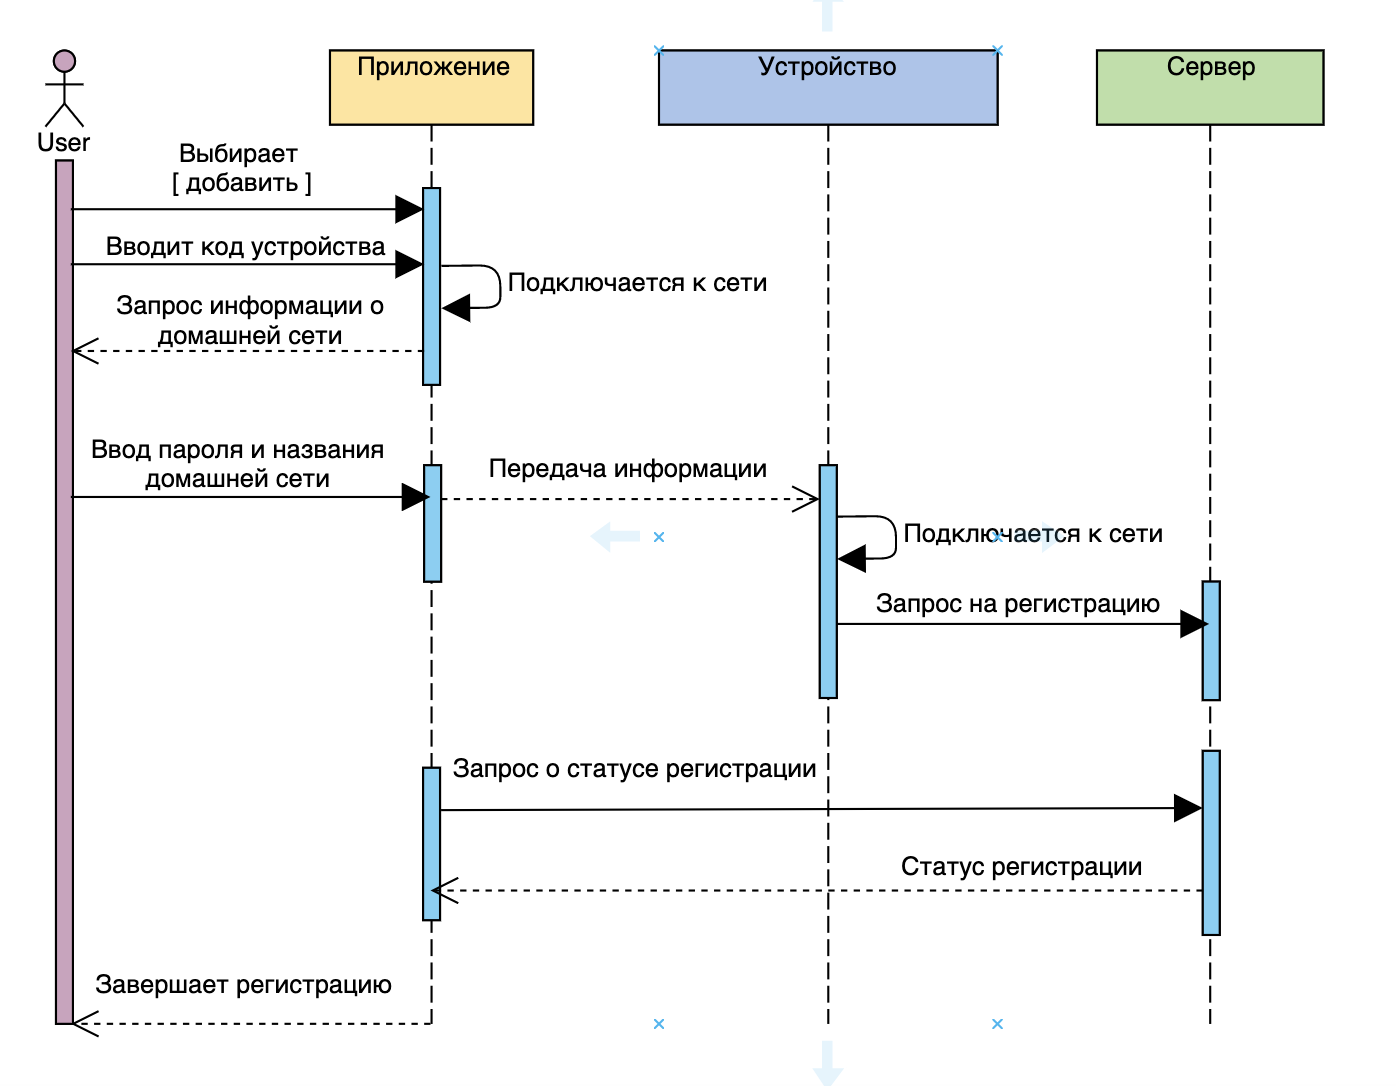
\includegraphics[scale=.5]{figures/pic_useCase1}
    \caption{UseCase 1}
    \label{fig:pic_useCase1}
\end{figure}

\subsection{Забыть устройство}
Пользователь может отвязать устройство от своего аккаунта. Например, если устройство больше не будет использоваться или в тех ситуациях, когда пользователь хочет привязать устройство к другому устройству.

Действующие лица	Устройство, Сервер, Пользователь, Приложение
Цель	Отвязать устройство от аккаунта пользователя
Условие	Пользователь ранее регистрировал устройство на свой аккаунт
Результат	Мобильное устройство забывает об устройстве, а устройство возвращается в изначальное состояние

Успешный сценарий (рисунок \ref{fig:pic_useCase2})
\begin{itemize}
    \item Пользователь выбирает удаление конкретного устройства
    \item Приложение отправляет устройству соответствующий запрос
    \item Приложение отправляет серверу соответсвующий запрос
    \item Приложение удаляет информацию об устройстве
    \item Приложение уведомляет пользователя об успешном завершении операции
\end{itemize}

\begin{figure}[ht]
   \centering
   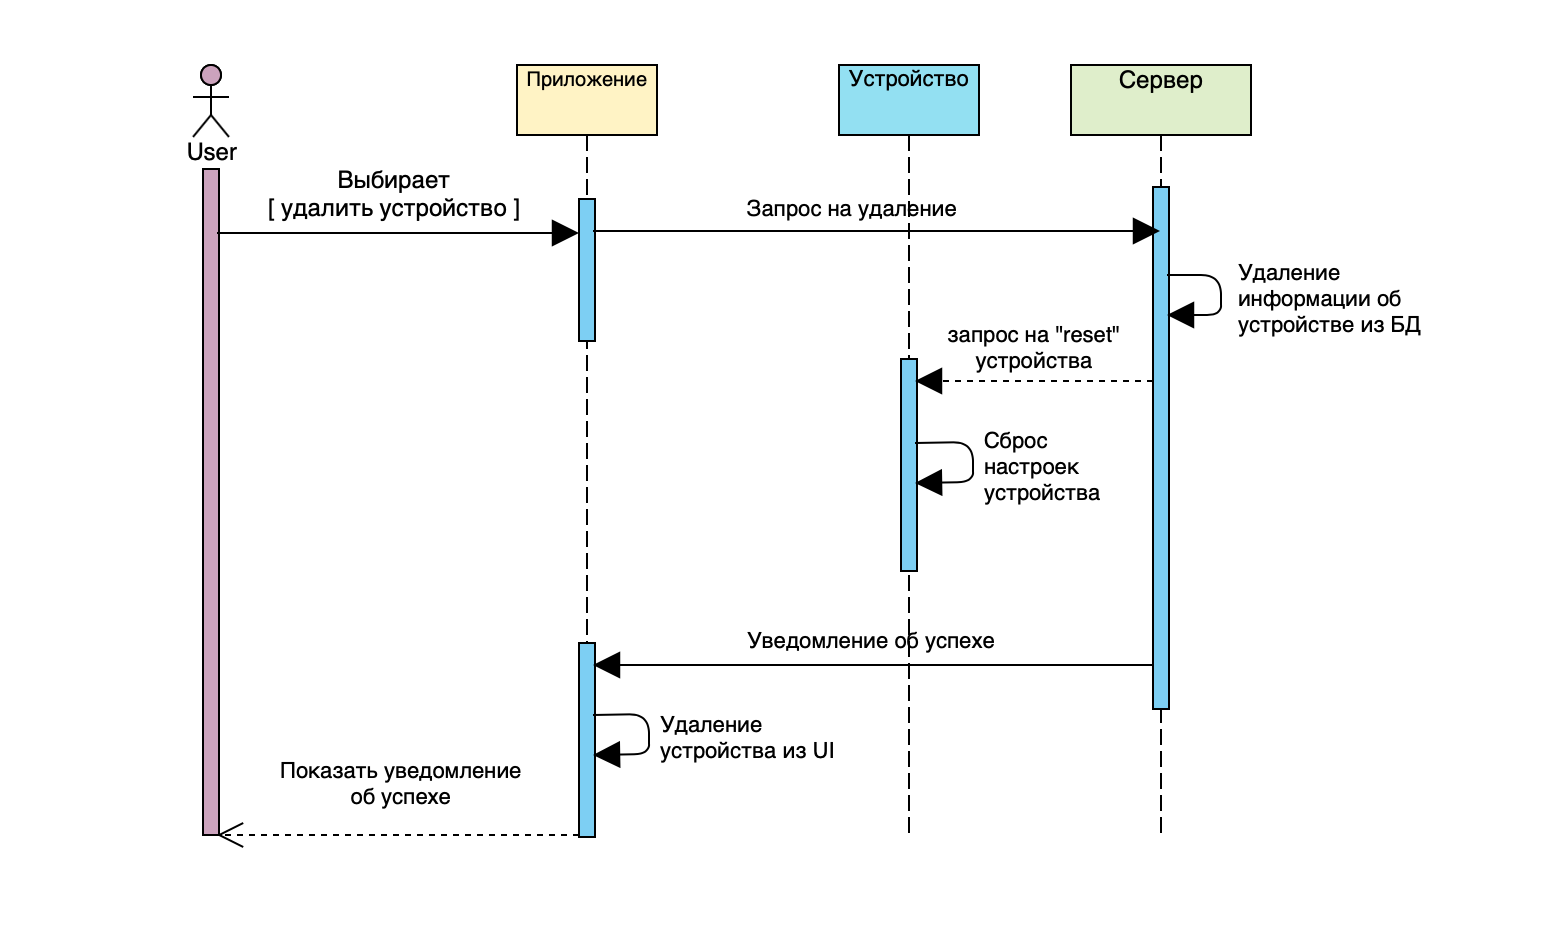
\includegraphics[scale=.5]{figures/pic_useCase2}
    \caption{UseCase 2}
    \label{fig:pic_useCase2}
\end{figure}

\subsection{Посмотреть список устройств управляемых с мобильного приложения}
Пользователь может посмотреть список устройств, которые он ранее зарегистрировал в мобильном приложении. Информация об устройствах хранится в базе данных мобильного устройства, которая обновляется из облака.

Описание сценария приведено на рисунке \ref{fig:pic_useCase3}.


    Для обновления информации о списке устройство на сервер делается HTTP запрос
    Приложение для каждого устройства должно отображать:
\begin{itemize}
    \item иконку, которая однозначно определяет тип устройства 
    \item название устройства
    \item уровень заряда (для устройств имеющих такой параметр)
    \item доступность устройства
    \item активное ли устройство.
\end{itemize}


\begin{figure}[ht]
   \centering
   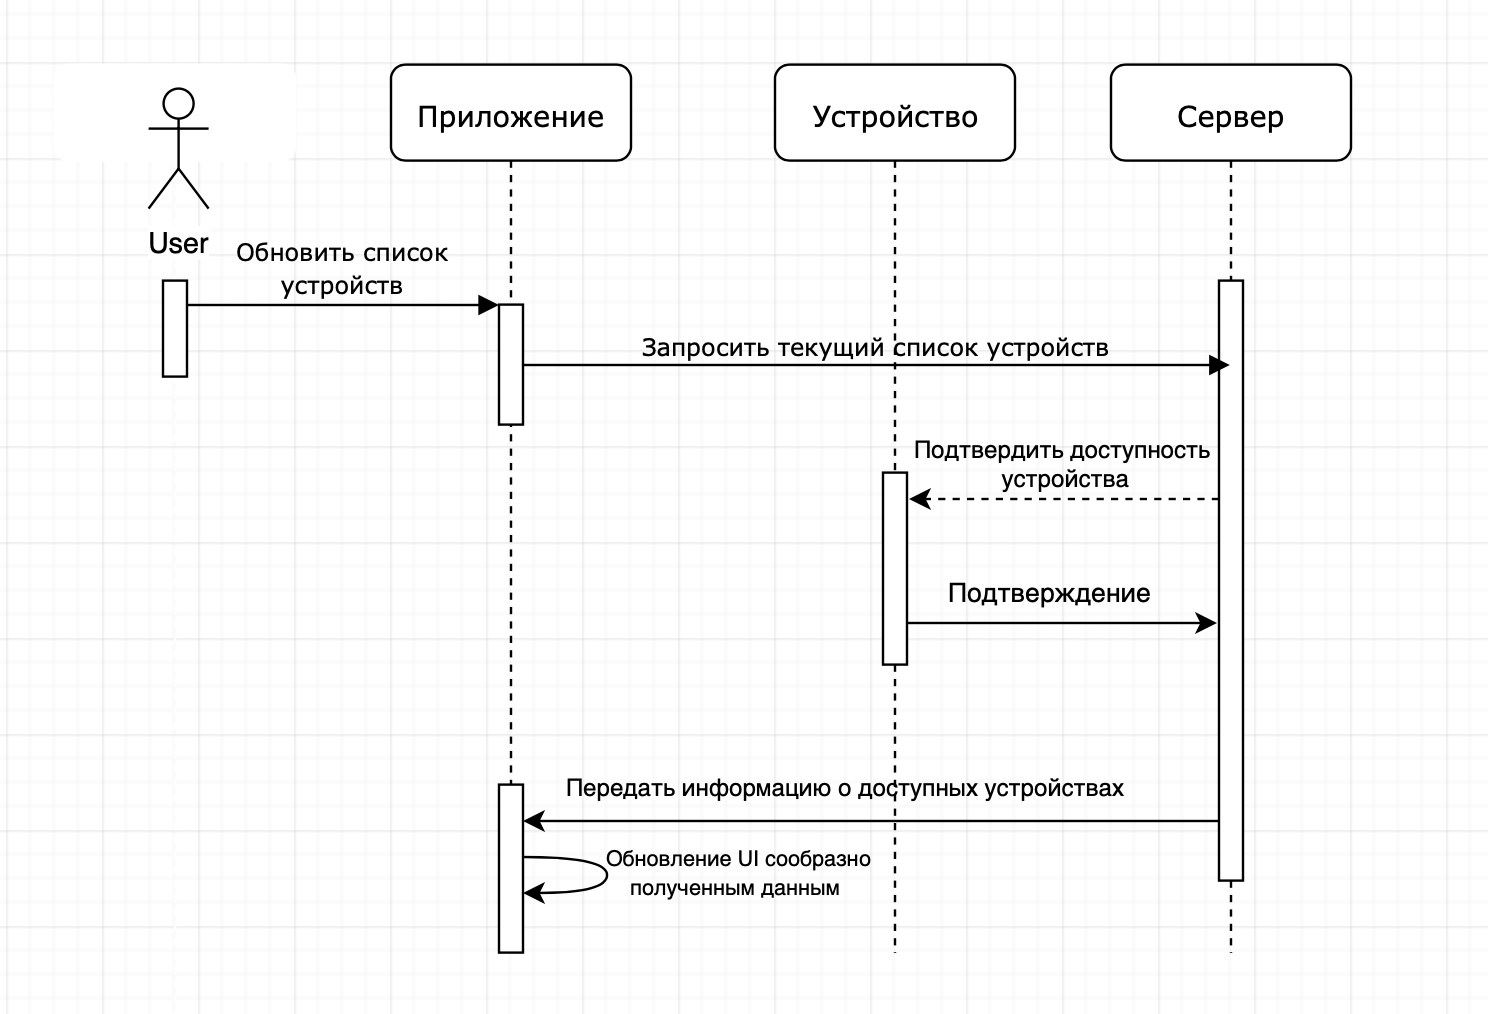
\includegraphics[scale=.5]{figures/pic_useCase3}
    \caption{UseCase 3}
    \label{fig:pic_useCase3}
\end{figure}

\subsection{Просмотр доступных сценариев}

Пользователь может просматривать доступные для установки на устройство сценария. Список сценариев хранится в базе данных устройства, которая обновляется из облака по запросу от мобильного приложения

Для обновления информации о списке доступных сценариев на сервер делается HTTP запрос

Приложение для каждого устройства должно отображать:
\begin{itemize}
 \item название сценария
  \item иконку сценария
\end{itemize}


\begin{figure}[ht]
   \centering
   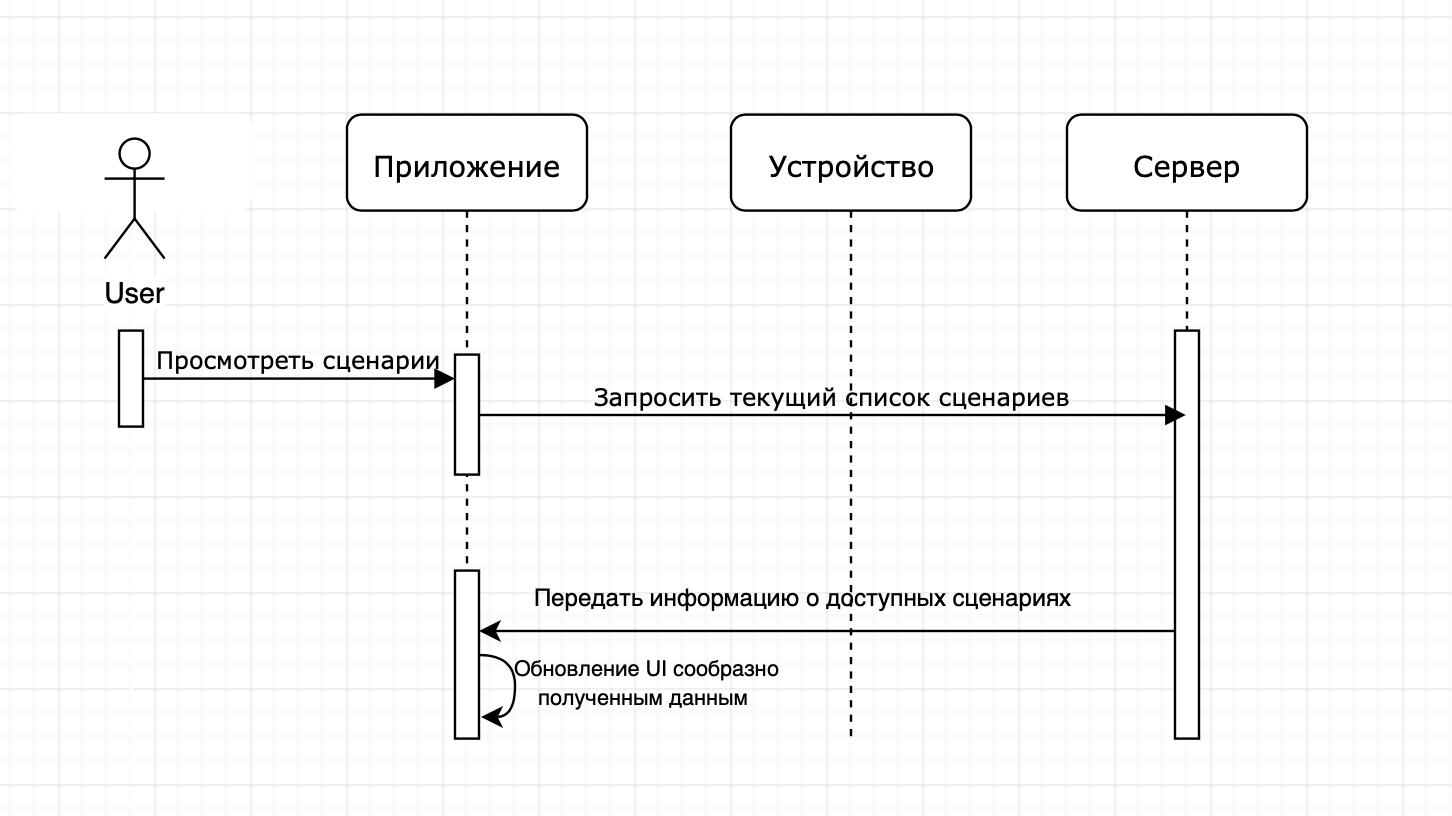
\includegraphics[scale=.5]{figures/pic_useCase4}
    \caption{UseCase 4}
    \label{fig:pic_useCase4}
\end{figure}

\subsection{Запуск сценария}  
Команда \verb|POST /device/<id>/scenario| - производит запуск сценария на устройстве с id=<id>. В качестве параметров передается JSON имеющий следующие поля:
\begin{itemize}
\item model - Тип String, модель осветительного устройства.
\item looped - Тип Bool, принимает значения:
true - если сценарий является зацикленным (то есть воспроизводящимся вновь по окончанию),
false - если сценарий не является зацикленным (то есть устройство не воспроизводит светомузыку по окончанию сценария)
\item method - Тип String, название метода, который нужно произвести с устройством. Может принимать два значения:
switch\_mod - На устройстве будет воспроизведен некоторый сценарий.
turn\_off - Устройство погаснет.
\item params - Тип Map, содержит описание сценария. См ниже Атрибуты сценария
\item brightness - Тип Float, яркость, принимает значения от 0 до 1.0
\item duration - Тип Int, длительность сценария в миллисекундах
\end{itemize}
Пример JSON:
\begin{verbatim}
request
{
 "model": "COSGarland_1",
 "looped": true,
 "method": "switch_mode",
 "params": [
  "mode": "double_color",
  "color1": "red",
  "color2": "white"
 ],
 "brightness": 0.5,
 "duration": 20,
}   
\end{verbatim}


\subsubsection{Атрибуты сценария}

Поле params содержит в себе основную информацию о сценарии, который будет воспроизведен. params содержит в себе:

mode - Тип String, название сценария. (Полный список сценариев см ниже Виды сценариев)

color1 - Тип String, Цвет 1, принимающий участие в светомузыке. Принимает значения: (red, green, white etc...)

color2 - Тип String, Цвет 2, принимающий участие в светомузыке. Принимает значения: (red, green, white etc...)

period - Тип Int, Некоторый период в миллисекундах. Играет разные роли в зависимости от параметра mode.

\subsubsection{Виды сценариев}

Ниже приведены некоторые из возможных режимов работы гирлянды:

solid\_color - Гирлянда горит одним цветом

double\_color - Гирлянда горит двумя цветами: четные лампочки горят цветом 1, а нечетные цветом 2

fading - Гирлянда затухает, а затем загорается с заданным периодом

blinking - Гирлянда мигает заданным цветом с заданным периодом

running\_light - Лампочки гирлянды загораются по очереди сменяя друг друга с заданным периодом

random - Гирлянда воспроизводит некую случайную последовательность световых сигналов


 
\section{Разработка API облачного сервера}
  
\section{Разработка формата описания сценариев работы ``умной гирлянды''}  

Нами разработан общий способ описания любого сценария RGB гирлянды. Он представляет из себя XML со следующими полями:

scenario - Внутри этого тэга находится вся информация о сценарии

mode\_name - Тип String, Имя описываемого сценария

one\_period\_duration - Тип Int, длительность между итерациями свечения гирлянды в миллисекундах (Через сколько времени лампочки должны сменить цвет)

number\_of\_periods - Тип Int, число описанных выше итераций

lamp - Объект содержащий в себе состояния цвета лампы. Содержит один атрибут - color, это цвет в формате RGB.

state - Описывает состояние всей гирлянды в данный момент времени. Имеет собственный ID соответсвующий порядковому номеру соответствующего момента времени.

\begin{verbatim}
<?xml version="1.0" encoding="UTF-8"?>
<?xml-stylesheet href="garland.xsl" type="text/xsl" ?>
<scenario>
    <mode_name>Double color running light mode</mode_name>
    <one_period_duration>300</one_period_duration> 
    <number_of_periods>11</number_of_periods> 
    <state id = '0'>
	    <lamp color = '#123d8c'/>
        <lamp color = '#000000'/>
        <lamp color = '#000000'/>
        <lamp color = '#7d69b5'/>
        <lamp color = '#000000'/>
	</state>
    <state id = '1'>
	    <lamp color = '#000000'/>
        <lamp color = '#123d8c'/>
        <lamp color = '#000000'/>
        <lamp color = '#000000'/>
        <lamp color = '#7d69b5'/>
	</state >
        ...
    <state id = '11'>
        <lamp color = '#000000'/>
        <lamp color = '#000000'/>
        <lamp color = '#7d69b5'/>
        <lamp color = '#000000'/>
        <lamp color = '#000000'/>
	</state >
</scenario>
\end{verbatim}
        % Описание  решения
%\chapter{Экспериментальная часть}
 \section{Функции мобильного приложения}
 Мобильное приложение, как часть системы умного освещения, выполняет следующие функции:
\begin{description}
	\item Предоставлять имя и пароль от локальной Wi-Fi сети для следующих устройств: гирлянда, манипулятор волшебная палочка; 
	\item Отображать текущие состояние устройства гирлянда, А именно:
	отображать активно ли устройство в данный момент времени (под активностью мы понимаем наличие доступа к сети интернет у устройства) (не реализовано), отображать последний момент времени, когда устройство было активно (не реализовано), отображать, от каких манипуляторов волшебная палочка гирлянда принимает команды (не реализовано);
	\item Отображать текущие состояние устройства манипулятор волшебная палочка. А именно:
	отображать активно ли устройство в данный момент времени, отображать уровень заряда аккумулятора, отображать последний момент времени, когда устройство было активно, отображать имена WiFi сетей, к которым <<волшебная палочка>> будет автоматически подключаться при обнаружении; 
	\item Отображать ассоциации для конкретной связки устройств: гирлянда - волшебная палочка;
	\item Реализовывать возможность добавления новых ассоциаций для конкретной связки устройств;
	\item Реализовывать возможность удаления ассоциаций для конкретной связки устройств (не реализовано);
	\item Управлять гирляндой через локальную Wi-Fi сеть. А именно: иметь возможность выключить и включить гирлянду, изменить цвет свечения гирлянды на выбранный пользователем (не реализовано), переключить режим свечения гирлянды на следующий, переключить режим свечения гирлянды на заданный пользователем (не реализовано), изменить цвет свечения гирлянды на случайный, задавать в реальном времени цвет свечения каждому световому диоду гирлянды по отдельности (не реализовано);
	\item Отображать в реальном времени жесты совершаемые манипулятором волшебная палочка;
	\item Реализовывать возможность создавать новый режим свечения гирлянды (не реализовано).
\end{description}
 \section{Разработка}
 В качестве среды разработки был выбран Xcode, язык программирования - Swift. В качестве архитектурного патерна был выбран патерн сходный с <<MVP>> (схема \ref{app-sceme-naked}). А именно: файлы с кодом были разделены на следующие логические блоки:
 \begin{description}
 \item [Model] представляет из себя модель данных, а именно: объект типа класс или структура хранящий информацию о чем-либо. Прямой доступ к Model имеет только Presenter. В приложении присутствует ряд объектов типа Model, реализующие модель хранения информации о состоянии следующих устройств: гирлянда, манипулятор волшебная палочка.
 \item [View] отвечает за отображение интерфейса и обработку действий, жестов произведенных пользователем в приложении. Обменивается информацией по изменению интерфейса с Presenter. На каждый <<экран>> в приложении приходится один класс типа View.
 \item [Presenter] отвечает за взаимодействие с данными. А именно: сохранение, редактирование, удаление данных. На каждый класс типа View в приложении приходится один класс типа Presenter. 
\item [Объекты, не укладывающиеся в архитектурный патерн]В проекте присутствуют вспомогательные классы и логические блоки необходимые для запросов в сеть интернет.
 \end{description}
 Объекты Model, View, Presenter и классы для интернет запросов имеют ряд связей описанных на схеме \ref{app-sceme-naked}. Ниже представленно подробное описание связей:
  \begin{description}
  \item [View $\Rightarrow$ Presenter] Класс View держит сильной ссылкой класс Presenter. Через эту связь View передает информацию о совершаемых пользователем действиях в Presenter.
  \item [Presenter $\Rightarrow$ Model] Класс Presenter держит сильной ссылкой класс Model. Через эту связь Presenter инициирует изменение переменных и других объектов класса Model.
  \item [Model $\Rightarrow$ Network] Класс Model держит сильной ссылкой класс, отвечающий за запросы в интернет. Через эту связь класс Model обновляет свои переменные и другие объекты, а также инициирует различные процессы в системе освещения - например, включение гирлянды.
  \item [Model $\Rightarrow$ Presenter] Класс Model держит слабой ссылкой класс Presenter. Через эту связь класс Model уведомляет Presenter об успешном совершении интернет запроса или об изменении своих переменных и других объектов.
  \item [Presenter $\Rightarrow$ View] Класс Presenter держит слабой ссылкой класс View. Через эту связь Presenter инициирует изменение визуальных объектов.
   \end{description}
 \begin{figure}[ht]
   \centering
   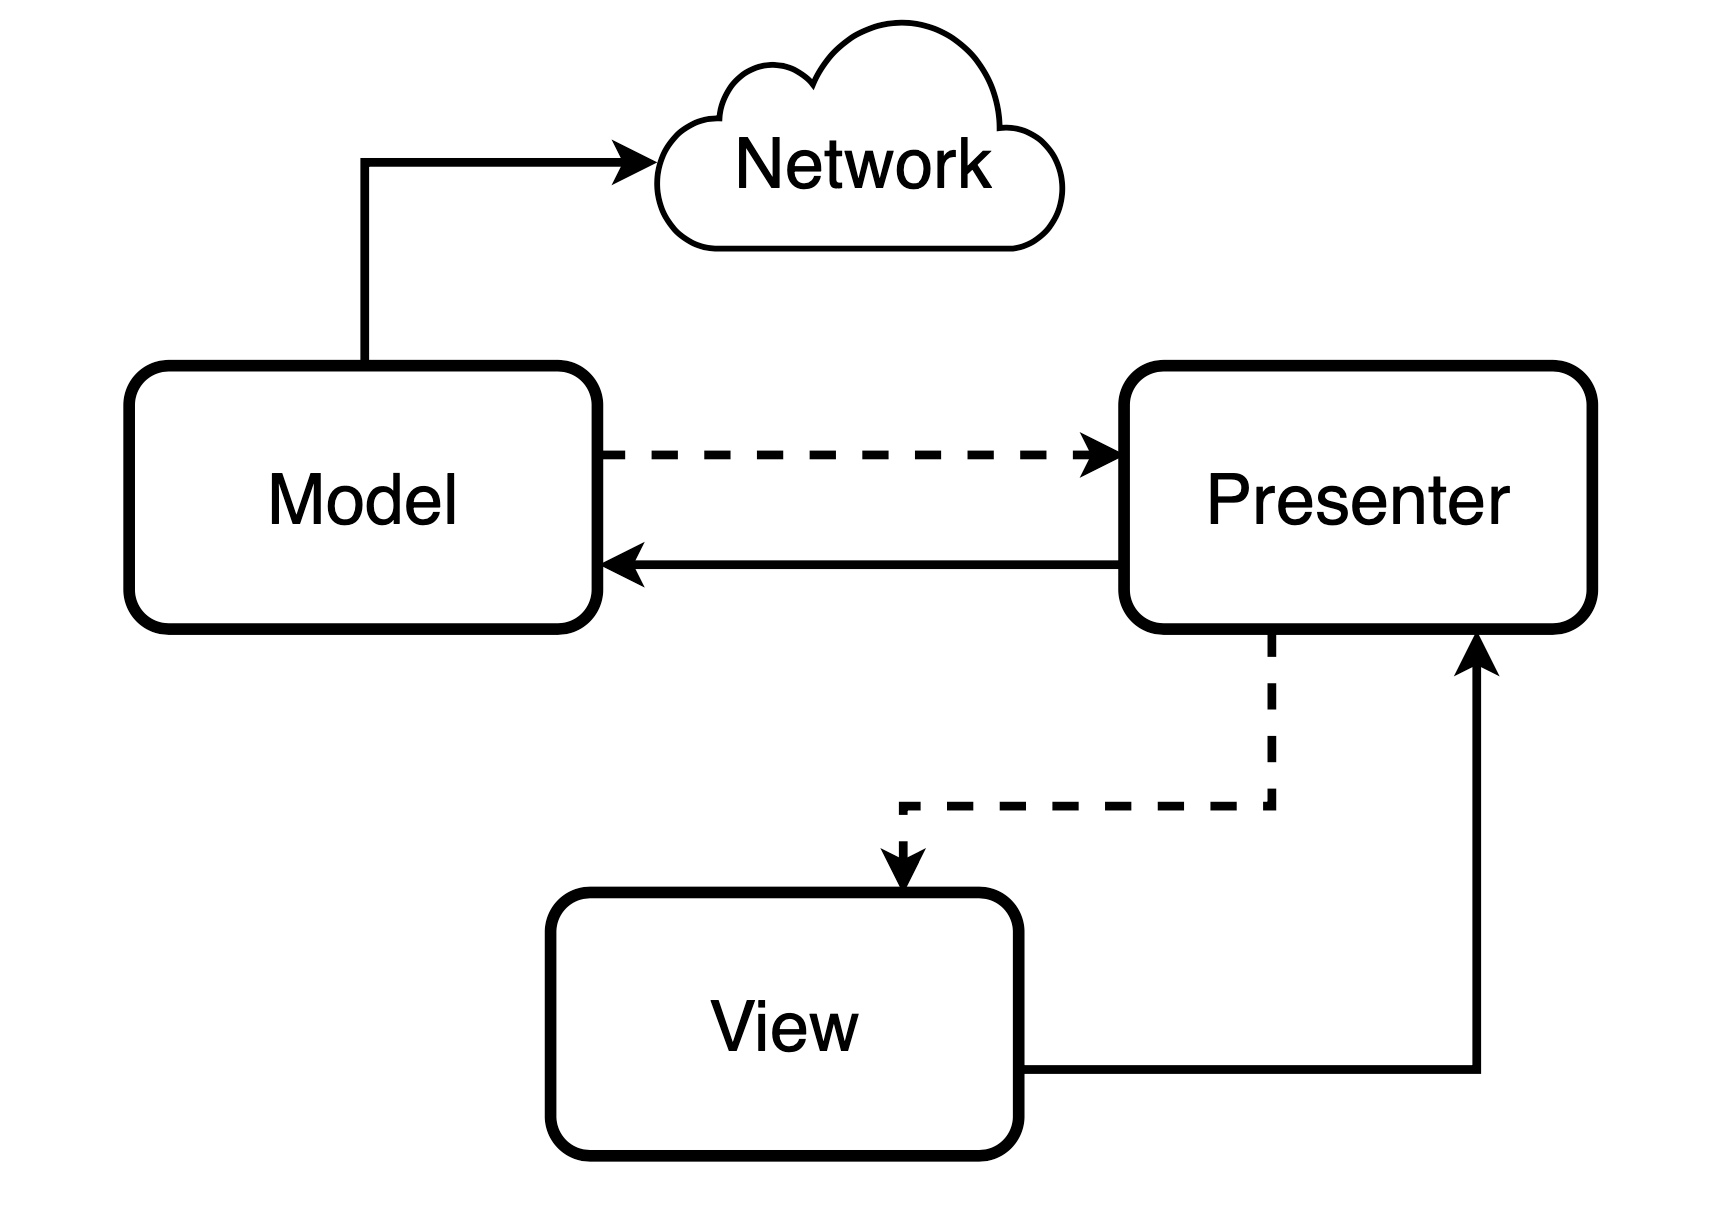
\includegraphics[scale=.25]{figures/mvp.jpg}
    \caption{Архитектурный патерн MVP}
    \label{mvp}
\end{figure}
  \section{Результат}
  Результат разработки описывается иерархией представлений (экранов) мобильного преложения (схема \ref{app-sceme-naked}).
  \begin{description}
  \item [Представление 1.1] Начальный экран, появляется сразу после открытия приложения. Содержит список устройств, а именно список гирлянд и манипуляторов <<волшебная палочка>>, которым был предоставлен доступ к локальному Wi-Fi. Также содержит кнопку <<Add new device>>, открывающую экран 2.1.
  \item [Представление 1.2] Экран настроек, пуст в текущей реализации.
  \item [Представление 2.1] Экран, содержащий элементы по управлению гирляндой. А именно:
  \begin{enumerate} 
    \item Переключатель для включения/выключения гирлянды
    \item Кнопка <<Switch mode>> меняющая режим свечения гирлянды на следующий
    \item Кнопка <<Random color>> меняющая цвет свечения гирлянды на случайный
\end{enumerate}
  \item [Представление 2.2] Экран для добавления нового устройства в список экрана 1.1. Имеет список устройств, доступных для добавления.
  \item [Представление 2.3] Экран, содержащий информацию о волшебной палочке в виде таблицы. А именно, таблица содержит следующие ячейки:
%   \renewcommand{\labelenumii}{\arabic{enumi}.\arabic{enumii}.}
\begin{enumerate} 
    \item Ячейка, отображающая активна ли волшебная палочка в данный момент
    \item Ячейка, отображающая насколько давно волшебная палочка была в сети
    \item Ячейка, отображающая уровень заряда аккумулятора
    \item Ячейка, отображающая список имен известных Wi-Fi сетей
   
    \item Ячейка, открывающая экран ассоциаций при нажатии
    \item Ячейка, открывающая экран жестов при нажатии
\end{enumerate}
Также содержит кнопку <<Update>>, обновляющую информацию в ячейках, описанных выше.
  \item [Представление 3.1] Экран, содержащий инструкцию по добавлению нового устройства. Отображает прогресс пользователя по выполнению инструкции.
    \item [Представление 3.2] Экран, содержащий ассоциации имеющиеся для данной волшебной палочки. Также содержит кнопку <<Add>>, открывающую экран 4.1.
    \item [Представление 3.3] Экран, в реальном времени отображающий жесты совершаемые волшебной палочкой.
    \item [Представление 4.1] Экран, реализующий создание новой ассоциации. Содержит меню выбора соответствий между жестом и действием. Также содержит кнопку <<Add>>, которая возвращает на экран 3.1. 
 \end{description}
 Имеются переходы между экранами в иерархии:
  \begin{description}
  \item [Переход 1.1 - 1.2] Осуществляется нажатием на правую часть меню в нижней части экрана (этот элемент имеет название tab bar). Так как tab bar доступен на всех экранах в иерархии, то и переход в настройки и обратно доступен везде. Таким образом помимо перехода 1.1 - 1.2, существуют аналогичные переходы: 1.2 - 1.1, 2.1 - 1.2, 1.2 - 2.1, 2.2 - 1.2 и тд. 
  \item [Переход 1.1 - 2.1] Осуществляется нажатием на ячейку типа <<гирлянда>> из списка доступных устройств.
  \item [Переход 1.1 - 2.2] Осуществляется нажатием на кнопку <<Add new device>> в верхней правой части
  \item [Переход 1.1 - 2.3] Осуществляется нажатием на ячейку типа <<волшебная палочка>> из списка доступных устройств.
  \item [Переход 2.2 - 3.1] Осуществляется нажатием на элемент типа <<гирлянда>> или типа <<волшебная палочка>> из списка устройств для добавления.
  \item [Переход 2.3 - 3.2] Осуществляется нажатием на ячейку ассоциаций - <<Associations>>.
  \item [Переход 2.3 - 3.3] Осуществляется нажатием на ячейку жестов - <<Moves>>.
  \item [Переход 3.1 - 1.1] Осуществляется автоматически после успешного выполнения пользователем всех пунктов инструкции. После выполнения перехода на экране 1.1 появляется только что добавленное устройсво.
  \item [Переход 3.2 - 4.1] Осуществляется нажатием на кнопку <<Add>> в верхней правой части.
  \item [Переход 4.1 - 3.2] Осуществляется нажатием на кнопку <<Add>> в верхней правой части. После выполнения перехода на экране 3.2 появляется только что созданная ассоциация.
  \item [Переходы навигации] На всех экранах второго и более уровней в иерархии представлений существует возможность вернуться на экран ниже, нажав на кнопку расположенную в верхней левой части экрана. Таким образом, все переходы, ведущие по иерархии вверх, обратимы. 
 \end{description}
\begin{figure}[ht]
   \centering
   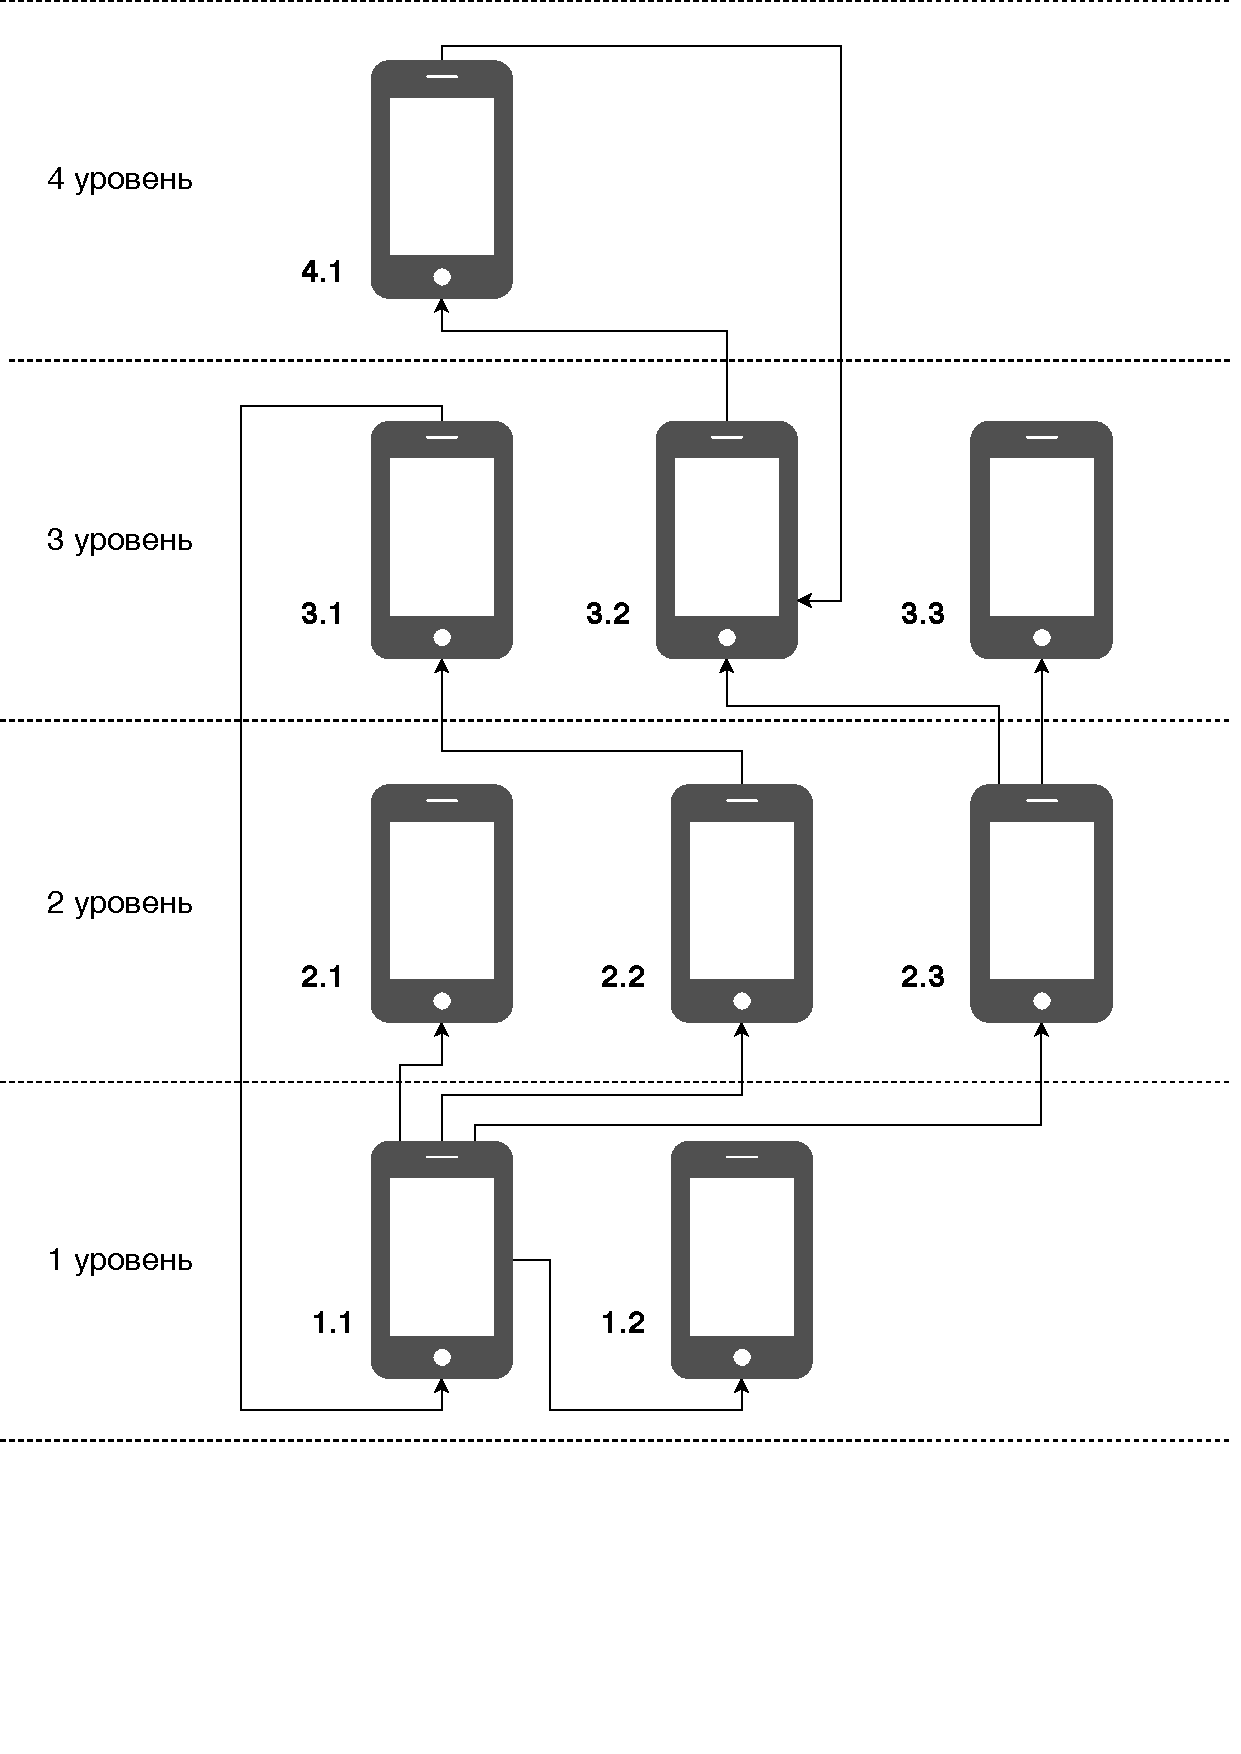
\includegraphics[scale=.75]{figures/app-sceme-naked.pdf}
    \caption{Иерархия представлений (экранов) в мобильном приложении}
    \label{app-sceme-naked}
\end{figure}
\label{cha:Experiment}
        % Описание результатов

%\chapter{Защита интеллектуальной собственности}
 \section{Формула изобретения}
 
1. Способ управления освещением заключающийся в том, что 

ставят в соответствие команды, передаваемые через локальную или глобальную сеть на устройство освещения управляющим командам, формируемым на устройстве управления освещением, 

формируют команды управления освещением,

определяют номера устройств и команды управления освещением

в соответствии с полученной командой управления формируют световую картинку одним или несколькими осветительными устройствами 

\textbf{отличающийся тем, что для формирования команд управления освещением }

выполняют жест устройством, содержащим компоненты регистрации ускорений,

регистрируют проекцию ускорения на некоторые выбранные оси в некоторых точках устройства - манипулятора как функцию времени,

преобразуют проекцию ускорения в массив данных, 

передают массив данных на облачный сервер,

вычисляют код жеста, поставленный в соответствие переданного массива данных,

определяют набор команд, которые должны быть активизированы по результатам определения жеста,

передают команды на осветительное устройство, 


 
 
2. Система управления освещением, реализующая способ управления освещением, включающая в себя:


устройство, имеющее название, включающее корпус, вычислительный модуль, модуль передачи данных по беспроводному каналу, модуль передачи данных (имеющий доступ в интернет),   

сервер, подключенный к сети интернет,

устройство, включающее корпус, вычислительный модуль, модуль передачи данных по беспроводному каналу, модуль передачи данных  (имеющий доступ в интернет),  

одно или несколько осветительных устройств, каждое из которых включает, вычислительный модуль, модуль передачи данных, один или несколько осветителей (ламп),


мобильный телефон с установленным на нем специальным мобильным приложением,

\textbf{при этом}



\textbf{отличающееся тем, что в состав системы управления освещением дополнительно включено}

устройство "волшебная палочка", включающее  вычислительный модуль,  один или несколько акселерометров и модуль передачи данных по беспроводному каналу, корпус,

\textbf{при этом }
модуль передачи данных по беспроводному каналу устройства "волшебная палочка" соединен по безвоздушной линии передачи данных с модулем передачи данных по беспроводному каналу устройства, включающее корпус, вычислительный модуль, модуль передачи данных по беспроводному каналу, модуль передачи данных  (имеющий доступ в интернет),

2. Система по пункту 1, отличающаяся тем, что два устройства, включающие корпус, вычислительный модуль, модуль передачи данных по беспроводному каналу, модуль передачи данных (имеющий доступ в интернет) объединены в один.


\section{Описание изобретения}

Изобретение "Способ управления освещением и система для его реализации" относится к коду H05B 37/02 МПК 

 
\subsection{Область техники, к которой относится изобретение}

Изобретение относится к области бытовых электрических приборов, в частности - к бытовым осветительным приборам.



\subsection{Раскрытие сущности изобретения}
1. Предложен способ управления освещением, заключающийся в том, что для управления "умным осветителем" разрабатывают набор команд управления состоянием осветительного устройства. 

В качестве такого устройства может использоваться, например "умная лампа" компании XIAOMI 

Она управляется командами через REST протокол.

При получении такой команды лампа светится синим цветом, соответствующим RGB тройке



ставят в соответствие команды, передаваемые через локальную или глобальную сеть на устройство освещения управляющим командам, формируемым на устройстве управления освещением, 

формируют команды управления освещением,

определяют номера устройств и команды управления освещением

в соответствии с полученной командой управления формируют световую картинку одним или несколькими осветительными устройствами 

\textbf{отличающийся тем, что для формирования команд управления освещением }

выполняют жест устройством, содержащим компоненты регистрации ускорений,

регистрируют проекцию ускорения на некоторые выбранные оси в некоторых точках устройства - манипулятора как функцию времени

преобразуют проекцию ускорения в массив данных, 

передают массив данных на облачный сервер

вычисляют код жеста, поставленный в соответствие переданного массива данных,

определяют набор команд, которые должны быть активизированы по результатам определения жеста,

передают команды на осветительное устройство, 



2. Предложена система управления освещением, включающая   
устройство 2, включающее корпус , вычислительный модуль, модуль передачи данных по беспроводному каналу, модуль передачи данных  (имеющий доступ в интернет),   

сервер 3, подключенный к сети интернет,

устройство 4, включающее корпус , вычислительный модуль, модуль передачи данных по беспроводному каналу, модуль передачи данных  (имеющий доступ в интернет),  

одно или несколько осветительных устройств 5,   каждое из которых включает, вычислительный модуль, модуль передачи данных, один или несколько осветителей (ламп),


мобильный телефон 6 с установленным на нем специальным мобильным приложением,

\textbf{при этом}



\textbf{отличающееся тем, что в состав системы управления освещением дополнительно включено}

устройство "волшебная палочка"  1, включающее  вычислительный модуль 1.1,  один или несколько акселерометров 1.2 и модуль передачи данных по беспроводному каналу 1.3, корпус,

\textbf{при этом }
модуль передачи данных по беспроводному каналу 1.3 устройства "волшебная палочка" соединен по безвоздушной линии передачи данных с модулем передачи данных по беспроводному каналу 2.2 устройства 2,

В качестве вычислительного модуля может быть использован вычислительный модуль на основе процессора 

В качестве акселерометра 1.2 может быть, например, использован акселерометрический блок 9250 компании Texas Instruments. 
 

\subsection{Краткое описание чертежей (если они содержатся в заявке)}
1. Система по пункту 1
На фиг.1 приведена блок схема описывающая способ управления освещением.

\begin{figure}[ht]
   \centering
   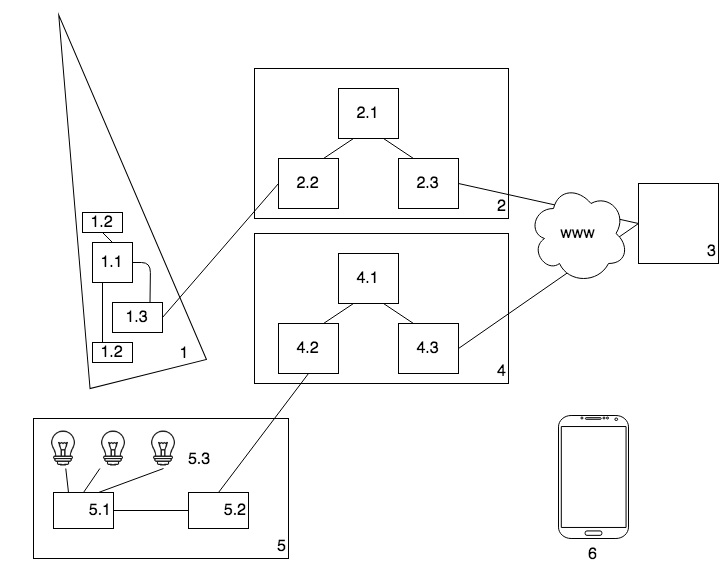
\includegraphics[scale=.4]{figures/patent-Magget-egor}
    \caption{Принципиальная схема системы 1}
    \label{patent-Magget-egor}
\end{figure}


Система включает 

устройство 2, включающее корпус , вычислительный модуль, модуль передачи данных по беспроводному каналу, модуль передачи данных  (имеющий доступ в интернет),   

сервер 3, подключенный к сети интернет,

устройство 4, включающее корпус , вычислительный модуль, модуль передачи данных по беспроводному каналу, модуль передачи данных  (имеющий доступ в интернет),  

одно или несколько осветительных устройств 5,   каждое из которых включает, вычислительный модуль, модуль передачи данных, один или несколько осветителей (ламп),


мобильный телефон 6 с установленным на нем специальным мобильным приложением,

\textbf{при этом}



\textbf{отличающееся тем, что в состав системы управления освещением дополнительно включено}

устройство "волшебная палочка"  1, включающее  вычислительный модуль 1.1,  один или несколько акселерометров 1.2 и модуль передачи данных по беспроводному каналу 1.3, корпус,

\textbf{при этом }
модуль передачи данных по беспроводному каналу 1.3 устройства "волшебная палочка" соединен по безвоздушной линии передачи данных с модулем передачи данных по беспроводному каналу 2.2 устройства 2,

На фиг.2  приведен пример сигнала на выходе акселерометра.

\begin{figure}[ht]
   \centering
   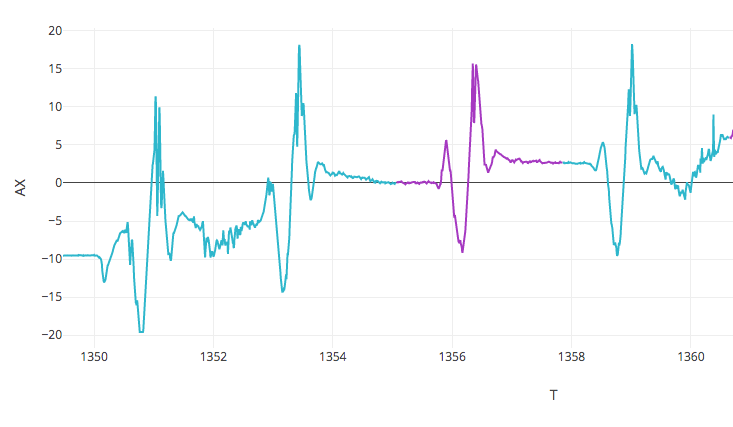
\includegraphics[scale=.5]{figures/AX-demo.png}
    \caption{Сигнал на выходе акселерометра}
    \label{fig:AX-data}
\end{figure}

%\begin{figure}[h]
 %  \centering
%   \includegraphics[scale=.4]{figures/fig2-accelerometer_data}
 %%%\end{figure}

2. Система по пункту 1, отличающаяся тем, что устройство 2 и устройство 4 совмещены.

\subsection{Осуществление изобретения}  

1. Способ управления освещением реализуется следующим образом.

Выполняют жест устройством 1, содержащим компоненты регистрации ускорений 1.2, регистрируют проекцию ускорения на некоторые выбранные оси в некоторых точках устройства - манипулятора как функцию времени. С помощью вычислительного модуля 1.1 преобразуют проекцию ускорения в массив данных. С помощью модуля передачи данных по беспроводному каналу 1.3 передают массив данных на облачный модуль передачи данных по беспроводному каналу 2.2 устройства 2. Массив данных, пройдя через вычислительный модуль 2.1, а затем через модуль передачи данных по беспроводному каналу 2.3 (имеющий доступ в интернет), передают на облачный сервер 3. Сервер снабжают нейронной сетью, способной вычислять код жеста, поставленный в соответствие переданного массива данных. Также на сервере определяют набор команд, которые должны быть активизированы по результатам определения жеста. Передается набор команд на осветительное устройство посредством устройства 4, аналогичным по своему составу устройству 2. Передают на осветительное устройство команды через модуль передачи данных 5.2. Затем данные через вычислительный модуль 5.1 распределяют по соответствующим данным лампочкам 5.3. Через лампочки  воспроизводят световой сигнал.

2. Система работает следующим образом.

При выполнении жеста, устройство 1, содержащее компоненты регистрации ускорений 1.2, регистрирует проекцию ускорения на некоторые выбранные оси в некоторых точках устройства - манипулятора как функцию времени. Вычислительный модуля 1.1 преобразуют проекцию ускорения в массив данных. Модуль передачи данных по беспроводному каналу 1.3 передает массив данных на облачный модуль передачи данных по беспроводному каналу 2.2 устройства 2. Массив данных, пройдя через вычислительный модуль 2.1, а затем через модуль передачи данных по беспроводному каналу 2.3 (имеющий доступ в интернет), приходит на облачный сервер 3. 

Сервер снабжен нейронной сетью, способной вычислять код жеста, поставленный в соответствие переданного массива данных. Также на сервере определяют набор команд, которые должны быть активизированы по результатам определения жеста. Устройство 4 передает набор команд на осветительное устройство посредством, аналогичным по своему составу устройству 2. Осветительное устройство, получает команды через модуль модуль передачи данных 5.2. Затем данные через вычислительный модуль 5.1 распределяются по соответствующим данным лампочкам 5.3. Лампочки воспроизводят световой сигнал.
 

 

\backmatter %% Здесь заканчивается нумерованная часть документа и начинаются ссылки и
            %% заключение

%\Conclusion % заключение к отчёту

По результатам работы решены следующие задачи:

\begin{itemize}
	\item изучено текущее состояние уровня техники в области ''умного освещения'';  
    \item разработана система команд для управления ''умной гирляндой''; 
    \item разработана архитектура взаимодействия ''умной гирлянды'', манипулятора волшебная палочка, сервера и мобильного приложения;
    \item  создана программная реализация мобильного приложения для управления ''умным домом'';
    \item  разработана заявка на патент на ''Способ управления освещением и устройство для его реализации''.
\end{itemize}

Конечным итогом проделанной работы является мобильное приложение.  

%%% Local Variables: 
%%% mode: latex
%%% TeX-master: "rpz"
%%% End: 
  % Выводы 

% % Список литературы при помощи BibTeX
% Юзать так:
%
% pdflatex rpz
% bibtex rpz
% pdflatex rpz

\bibliographystyle{gost780u}
\bibliography{smartlight}

%%% Local Variables: 
%%% mode: latex
%%% TeX-master: "rpz"
%%% End: 
      % Список литературы 

\pagestyle{empty} % нумерация выкл.
\chapter{ОТЗЫВ}
\textbf{на работу студента СОЛОВЬЕВА Е.А.}

Соловьев Е.А. проходил дипломную практику в ООО “Лаборатория моделирования систем” с сентября 2019 года.  

Тема дипломной работы - «Разработка технологии управления распределенной системой “умного освещения” с элементами искусственного интеллекта» связана с решением задачи построения систем класса smart home, при построении которых используется широкий спектр устройств (исполнительных, интерфейсных, инфраструктурных), платформ для их взаимодействия и приложений. Егору была поставлена задача сопряжения манипулятора “волшебная палочка” и устройства “новогодняя гирлянда” с помощью приложения на мобильном телефоне. 

Егор является основным исполнителем по данной теме и сумел освоить как аппаратную часть, так и осуществить программную реализацию в виде прототипа приложения для устройств iOS.  

Все поставленные в рамках работ задачи успешно выполнены. Уровень выполненной работы и имеющийся план дальнейшего развития проекта позволяют сформулировать задачу для написания магистерской диссертации.  

За время работы Егором разработан прототип приложения для мобильных телефонов iOS, позволяющий сопрягать манипулятор “волшебная палочка” с исполнительными устройствами.  

Работа предоставлена в срок.  

К недостаткам работы можно отнести отсутствие анализа при выборе архитектур примененных в работе.  

На основании вышеизложенного рекомендую оценить работу оцен кой «отлично», а СОЛОВЬЕВА Егора Александровича рекомендовать к поступлению в магистратуру МФТИ.
	
 \begin{tabular}{p{200pt}p{100pt}p{100pt}} \\[10pt]
        Научный руководитель доцент & &~А.В.Хельвас\\  
    \end{tabular}    

\appendix   % Тут идут приложения

 \chapter{XSL стиль для формирования отображения сценариев работы ``умной гирлянды''}
\label{cha:appendix1}


\begin{verbatim}
 <xsl:stylesheet version="1.0"
   xmlns:xsl="http://www.w3.org/1999/XSL/Transform"
   xmlns="http://www.w3.org/2000/svg">

<!-- Число периодов. Считывается из xml. -->
<xsl:param name="number_of_iterations">
  <xsl:for-each select="scenario">
      <xsl:value-of select="number_of_periods"/>
  </xsl:for-each>
</xsl:param>

<!-- Размер квадратной ячейки.--> 
<!--Рассчитывается изходя из количества периодов-->
<xsl:param name="cell_size">
 <xsl:if test="22 &lt; $number_of_iterations ">
      <xsl:value-of select="900 div $number_of_iterations"/>
 </xsl:if>
  <xsl:if test="$number_of_iterations &lt;= 22 ">
    <!-- Значение по умолчанию, если периодов мало.-->
    <xsl:value-of select="40"/>
 </xsl:if>
</xsl:param>

<!-- Название описываемого мода (сценария) -->
<xsl:param name="mode_name">
  <xsl:for-each select="scenario">
      <xsl:value-of select="mode_name"/>
  </xsl:for-each>
</xsl:param>

<!-- Длительность одного периода -->
<xsl:param name="one_period_duration">
  <xsl:for-each select="scenario">
      <xsl:value-of select="one_period_duration"/>
  </xsl:for-each>
</xsl:param>

<xsl:output method="xml" indent="yes" />
<xsl:template match="/">
   <html>
   <body>
   <h2><xsl:value-of select="$mode_name" /></h2>
   <h4>По оси x распологаются блоки временных периодов
   длительностью в <xsl:value-of select="$one_period_duration" /> 
   миллисекунд 
   <br />
   По оси y расположены блоки обозначающие лампы. 
   (n - порядковый номер лампы)
   </h4>
   <table border="1">
     
     <tr bgcolor="#9acd32">
      <!-- Заполнение верхней ячейки таблицы. -->
     <th width="{$cell_size}">n/t</th>
      
      <!-- Заполнение первого столбца номрами ламп. -->
      <xsl:call-template name="while_alowed_add_cell">
				<xsl:with-param name="VALUE" select="0"/>
			</xsl:call-template>
     </tr>

     <xsl:for-each select="scenario/lamp">
     <tr>
     <!-- Заполнение первой строки номерами итераций. -->
     <th bgcolor='#9acd32'><xsl:value-of select="@id"/></th>
     <!-- Заполнение таблицы. -->
     <xsl:for-each select="state">
      <td width="{$cell_size}" height ="{$cell_size}" 
      bgcolor='{@color}'></td>
     </xsl:for-each>
     </tr>
     </xsl:for-each>
   </table>
   </body>
   </html>
</xsl:template>

<!-- Заполяняет столбец цифрами от VALUE до number_of_iterations -->
<xsl:template name="while_alowed_add_cell">
 <xsl:param name="VALUE"/>

  <th height ="{$cell_size}" width="{$cell_size}"> 
   <xsl:value-of select="$VALUE" /> 
  </th>

 <xsl:if test="$VALUE != $number_of_iterations - 1">
      <xsl:call-template name="while_alowed_add_cell">
				<xsl:with-param name="VALUE" select="$VALUE + 1"/>
			</xsl:call-template>
 </xsl:if>
</xsl:template>

</xsl:stylesheet> 

\end{verbatim}
% \chapter{Еще картинки}
\label{cha:appendix2}

\begin{figure}
\centering
\caption{Еще одна картинка, ничем не лучше предыдущей. Но надо же как-то заполнить место.}
\end{figure}

%%% Local Variables: 
%%% mode: latex
%%% TeX-master: "rpz"
%%% End: 




\end{document}

%%% Local Variables:
%%% mode: latex
%%% TeX-master: t
%%% End:
